\section{Systematic uncertainties}
\label{sec:systematics}

This section describes the main sources of systematic uncertainties considered.
Other sources, which would matter in measurements of absolute quantities,
cancel in the ratio between the rare and resonant channels.
%
A list of the systematic uncertainties that are considered and their effect on the $R_{\Kstarz}$
ratio is summarised in Tab.~\ref{tab:systematics}.
The total uncertainty is evaluated by summing in quadrature the single components.

\begin{table}[h!]
\begin{center}
\caption{Summary of the relative systematic uncertainties on \RKst (in percentage).}
\renewcommand\arraystretch{1.4}
\label{tab:systematics}
\begin{tabular}{c|c|c}
\textbf{Source} & central-\qsq & high-\qsq\\ \hline

Signal shape		  		& 0.1      	& 0.2 \\
Bremsstrahlung categories 	& -- (??) 		& 0.2 \\
%Trigger categories 			&   		&  \\

\hline

ID swap			  		& 0.2	      & 0.1 \\
$\Lb\to pK\jpsi(\to \ll)$ 		& 0.8	      & 2.2 \\
$\Bs\to\Kstarz\jpsi(\to \ll)$		& 0.2	      & 0.1 \\

Mis-reconstructed	  		& 1.5     	&  -- \\
$\Lb\to pK\jpsi(\to \ll)$ 		& --	      	& -- \\
Combinatorial 		  		& 0.1	      	& 5.4 \\

$\Bz\to\Kstarz\jpsi(\to \ll)$ leakage      	& 0.3      & -- \\
$\Bz\to\Kstarz\psitwos(\to \ll)$ leakage      & 0.1      & 3.2 \\

\hline

\texttt{RooKeysPdf} ($\rho=1.1$)      & 0.2      & 0.3 \\
\texttt{RooKeysPdf} ($\rho=1.3$)      & 0.2      & 0.4 \\

\hline

Efficiency		  	& 0.4	      & 0.8 \\
TISTOS	          	& 2.3	      & 2.8 \\
Bin migration	  	& 		&   \\

\hline

Total				& 	      &  \\

\end{tabular}
\end{center}
\end{table}


\subsection{Choice of signal and background PDFs}

There is a certain arbitrariety in the choice of PDFs to model signal and background contributions in the
invariant mass fits, which could translate in a bias on the final result. The systematic uncertainty due to the
parameterisation of line shapes is studied in the following ways.

For the signal PDF:
%
\begin{itemize}

\item \textit{Shape}: in the electron channels the PDF is changed from a Crystal Ball and Gaussian to a Double Crystal Ball.
Modifying the PDF has a negligible effect in the muon modes but it affects the electron ones resulting in a $\sim 0.1\%$
variation on \RKst.

\item \textit{Bremsstrahlung categories}: gaussian constraints are applied to the relative fractions of the bremsstrahlung
categories, instead of fixing them to the values observed on simulation.
This yields a $\sim \%$ systematic on \RKst in the central- and high-\qsq region.

%\item \textit{Trigger categories}: the fit is repeated without splitting the electron sample in trigger categories;
%this results in a $\sim \%$ ($\sim \%$) variation on \RKst in the central-\qsq (high-\qsq) region;

\end{itemize}

For the background PDFs:
%
\begin{itemize}

\item \textit{ID swap}: a component that describes candidates where the particle identities are swapped
is added both to the muon and electron resonant fits, and constrained to the number of candiates
expected from simulation. This amounts to a $\sim \%$ variation on \RKst in the central- and high-\qsq region.

\item $\Lb\to pK\jpsi(\to \ee)$: the normalisation is left free to vary.
This results in a $\sim \%$ variation on \RKst in the central- and high-\qsq region.

\item $\Bs\to\Kstarz\jpsi(\to \ll)$: the $\Bs\to\Kstarz\jpsi(\to \mumu)$ shape is taken from simulation
instead of using the same shape as for the signal. The normalisation is fixed
to the branching ratio times the production fraction.
This results in a $\sim \%$ variation on \RKst in the central- and high-\qsq region.

\item \textit{Mis-reconstructed}: the yield of the mis-reconstructed background to \BdToKstee is left free to vary in the fit.
This only applies to the central-\qsq interval as this contribution is already free to vary in the high-\qsq range.
This yields a $\sim \%$ systematic on \RKst.

\item \textit{Combinatorial}: the PDF at high-\qsq is changed from an exponential (anti-MVA cut) to an anti-MVA
cut (exponential) for the $\mu\mu$ ($ee$) mode. This amounts to a $\sim \%$ variation on \RKst in the central- and high-\qsq region.

\item $\Lb\to pK \ll$: this background is added to the fit to the rare channel and returns zero yield for both the muon and the electron samples.
Therefore this yields no systematic uncertainty.

\item \textit{Leakage}: gaussian constraints are applied to the amounts of \BdToKstJPsee leakage in the central-\qsq region
 and to the $\Bz\to\Kstarz(\psitwos\to \ee)$ leakage in the high-\qsq region, which are fixed in the default fit.
This results in a $\sim \%$ variation on \RKst in the central- and high-\qsq region.

\end{itemize}


\subsection{Efficiency determinations}

The statistical uncertainty on the efficiency determinations is taken as the corresponding systematic uncertainty.
The correlation among the electron trigger categories is taken into account (e.g. L0E and L0H are anti-correlated).
This amounts to a $\sim \%$ ($\sim \%$) systematic uncertainty on \RKst for the central-\qsq (high-\qsq) interval.

A further source of systematic uncertainty associated to the trigger efficiency is estimated using the data-simulation
differences observed in Sec.~\ref{sec:tistos}. Ratios of efficiencies for the rare to resonant decays are found to be 
compatible between the electron and muon modes, indicating that the effect on \RKst is negligible, but the statistical 
precision on the determinations is taken as an extra systematic uncertainty.

%A further source of systematic, which is considered, is due to the
%discrepancies found in Sec.~\ref{sec:tistos} on the determination of the trigger efficiency. 
%As explained in that subsection the efficiency is derived as a function of the relevant
%kinematic quantities for each trigger category. The efficiency
%is then obtained for the rare and resonant sample by a weighted average.
%These are found to be compatible indicating that the effect on the
%ratios between rare and resonant channels is negligible.
%Therefore, no systematic uncertainty is added for this source.

\subsection{Bin migration}

The determination of the reconstruction efficiency is affected by the knowledge of the
amount of bin migration as explained in Sec.~\ref{sec:reco_binmig}. This amount depends
on the shape of the \qsq distribution, which in turn depends on the simulated \BdToKstee decay model.
In order to asses this systematic, simulated samples are generated using different
models corresponding to different form factors~\cite{Ball:2004ye,Melikhov:2000yu}.
The \qsq distributions obtained using each model are compared with the ones obtained using
the default one~\cite{Ali:1999mm}.
Figure~\ref{fig:q2ratios} shows normalised ratios between these \qsq distributions and the default one, 
which are used to re-weight the simulation. The amount of bin migration is recalculated
using the simulation reweighted to reproduce each model; Table~\ref{tab:sys_binmig} lists the
percent variations obtained. The largest difference between two values is taken as systematic uncertainty.
This results in a $\sim5\%$ uncertainty for the central-\qsq interval and $\sim11\%$ for the high-\qsq one,
which represent in both channel the biggest systematic uncertainty.
%
\begin{figure}[h!]
\centering 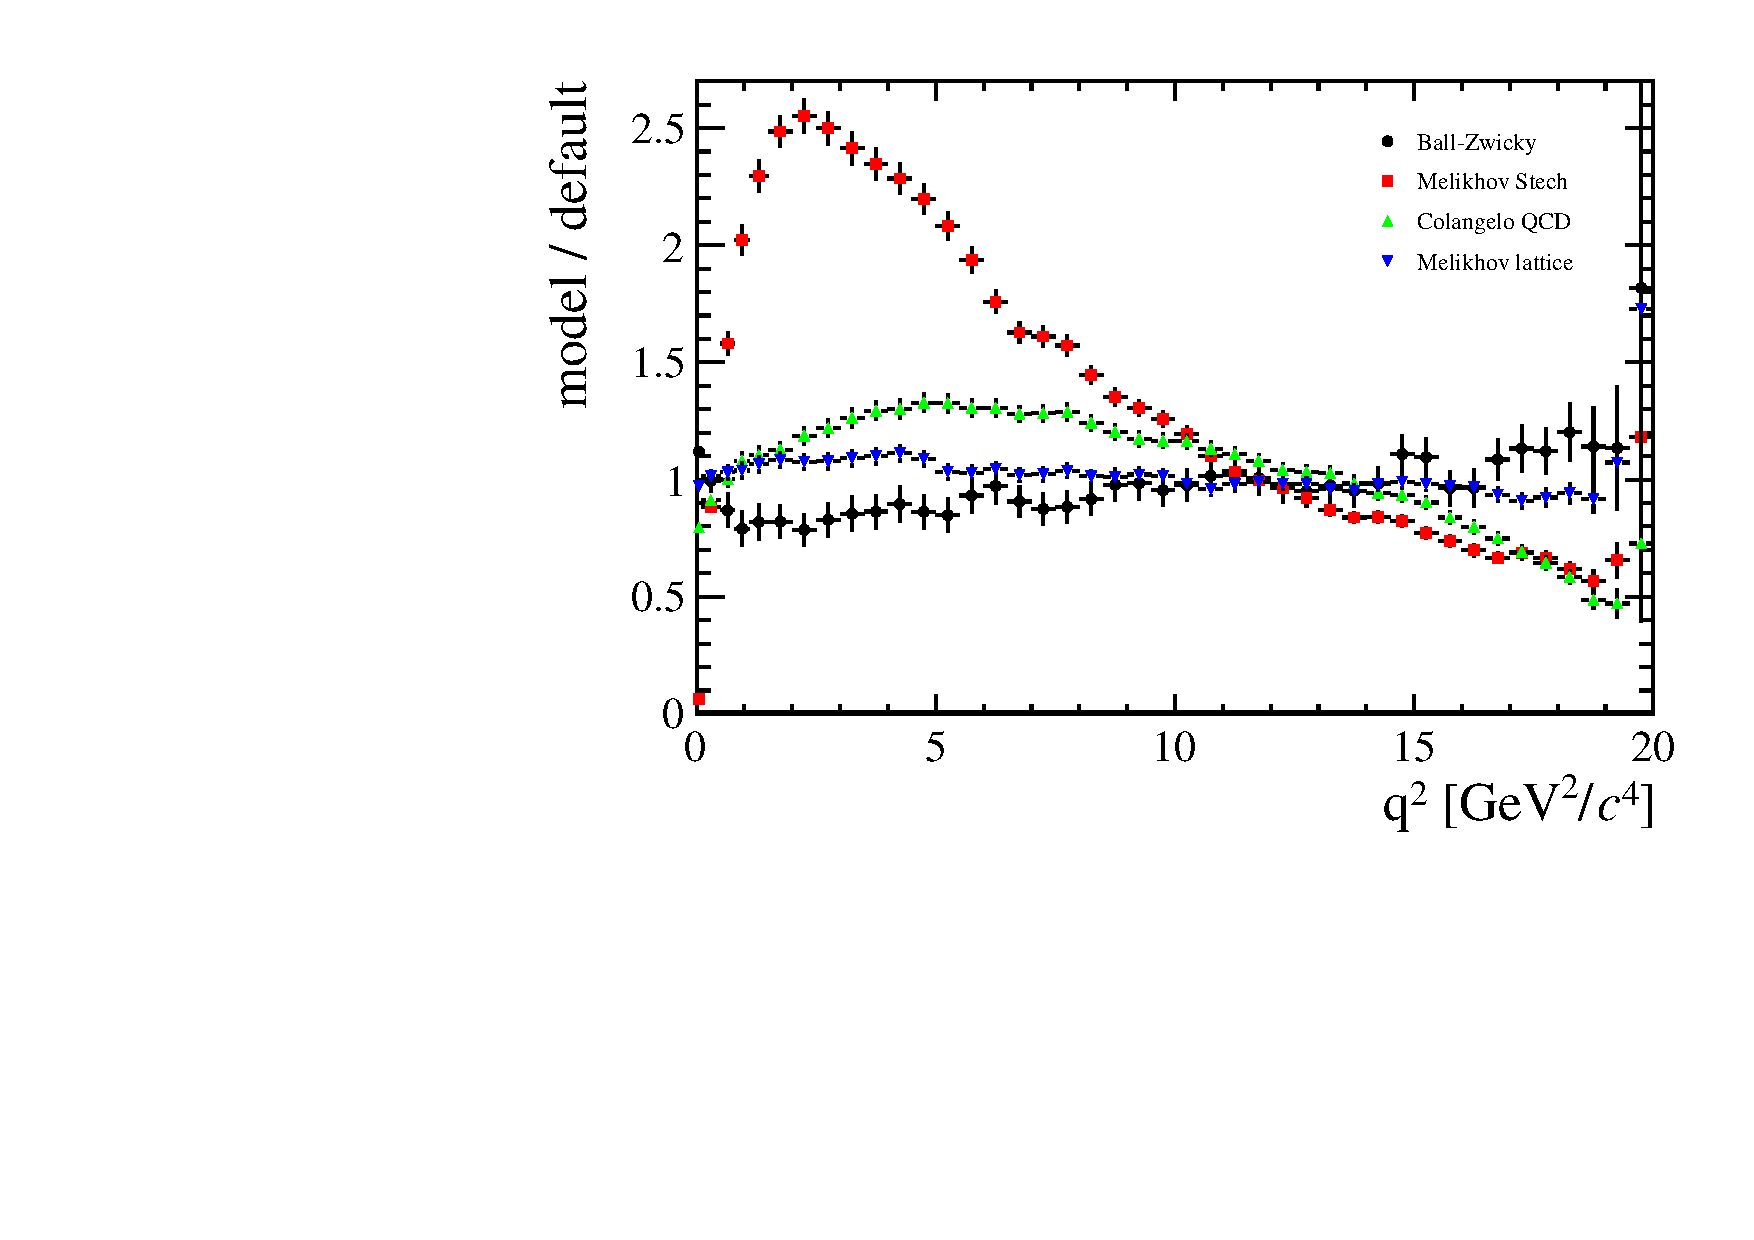
\includegraphics[width=0.8\textwidth]{RKst/figs/models_ratios.pdf}
\caption{Ratios between the \qsq distributions obtained using different form
factors models with respect to the default model. }
\label{fig:q2ratios}
\end{figure}
%
\begin{table}[h!]
\centering
\caption{Percent variation on the bin migration amount obtained using different form factors models.}
\begin{tabular}{|c|c|c|}
\hline
Model                   & 1--6 GeV$^2/c^4$  &  15--20 GeV$^2/c^4$ \\ \hline
Ball-Zwicky (6)         & 1.8          & 0.2    \\
Melikhov-Stech          & -3.7          & 6.6    \\
Colangelo QCD (3)   & 0.3           & 0.8    \\
Melikhov lattice  (4)   & -0.5          & -0.4    \\
\hline 
\end{tabular}
\label{tab:sys_binmig}
\end{table}




